\newcommand{\chunkNumber}[1]{\ensuremath{\mathsf{chunkNumber}(#1)}}
\newcommand{\relativeSlot}[2]{\ensuremath{\mathsf{relativeSlot}(#1, #2)}}

\chapter{Immutable Database}
\label{immutable}

The Immutable DB is tasked with storing the blocks that are part of the
\emph{immutable} part of the chain. Because of the nature of this task, the
requirements and \emph{non-requirements} of this component are fairly specific:

\begin{itemize}
\item \textbf{Append-only}: as it represents the immutable chain, blocks will
  only be appended in the same order as they are ordered in the chain. Blocks
  will never be \emph{modified} or \emph{deleted}.
\item \textbf{Reading}: the database should be able to return the block or
  header stored at a given \emph{point} (combination of slot number and hash)
  efficiently.\todo{define point somewhere?}
\item \textbf{Efficient streaming}: when serving blocks or headers to other
  nodes, we need to be able to stream ranges of \emph{consecutive} blocks or
  headers efficiently. As described in \cref{serialisation:network:serialised},
  it should be possible to stream \emph{raw} blocks and headers, without
  serialising them.
\item \textbf{Recoverability}: it must be possible to validate the blocks stored
  in the database. When a block in the database is corrupt or missing, it is
  sufficient to truncate the database, representing an immutable chain, to the
  last valid block before the corrupt or missing block. The truncated blocks can
  simply be downloaded again. It is therefore not necessary to be able recover
  the full database when blocks are missing.
\end{itemize}

While we touched upon some of the non-requirements already above, it is useful
to highlight the following non-requirements.

\begin{itemize}
\item \textbf{Queries}: besides looking up a single block by its point and
  streaming ranges of consecutive blocks, the database does have to be able to
  answer queries about blocks. No searching or filtering is needed.
\item \textbf{Durability}: the system does not require the durability guarantee
  that traditional database systems provide (the D in ACID). If the system
  crashes right after appending a block, it is acceptable that the block in
  question is truncated when recovering the database. Because of the overlap
  with the Volatile DB\todo{link}, such a truncation is likely to even go
  unnoticed. In the worst case, the truncated blocks can simply be downloaded
  again.
\end{itemize}

Because of the specific requirements and non-requirements listed above, we
decided to write our own implementation, the \lstinline!ImmutableDB!, instead of
using an existing off-the-shelf database system. Traditional database systems
provide guarantees that are not needed and, conversely, do not take advantage of
the requirements to optimise certain operations. For example, there is no need
for a journal or flushing (\lstinline!fsync!) the buffers after each write
because of our unique durability and recoverability (non-)requirements.

\section{API}
\label{immutable:api}

Before we describe the implementation of the Immutable DB, we first describe its
functionality. The Immutable DB has the following API:

\begin{lstlisting}
data ImmutableDB m blk = ImmutableDB {
      closeDB :: m ()

    , getTip :: STM m (WithOrigin (Tip blk))

    , appendBlock :: blk -> m ()

    , getBlockComponent ::
           forall b.
           BlockComponent blk b
        -> RealPoint blk
        -> m (Either (MissingBlock blk) b)

    , stream ::
           forall b.
           ResourceRegistry m
        -> BlockComponent blk b
        -> StreamFrom blk
        -> StreamTo   blk
        -> m (Either (MissingBlock blk) (Iterator m blk b))
    }
\end{lstlisting}

The database is parameterised over the block type \lstinline!blk! and the monad
\lstinline!m!, like most of the consensus layer.\todo{mention io-sim}
\todo{TODO} Mention our use of records for components?

The \lstinline!closeDB! operation closes the database, allowing all opened
resources, including open file handles, to be released. This is typically only
used when shutting down the entire system. Calling any other operation on an
already-closed database should result in an exception.

The \lstinline!getTip! operation returns the current tip of the Immutable DB.
The \lstinline!Tip! type contains information about the block at the tip like
the slot number, the block number, the hash, etc. The \lstinline!WithOrigin!
type is isomorphic to \lstinline!Maybe! and is used to account for the
possibility of an empty database, i.e., when the tip is at the ``origin'' of the
chain. This operation is an \lstinline!STM! operation, which allows it to be
combined with other \lstinline!STM! operations in a single transaction, to
obtain a consistent view on them. This also implies that no IO or disk access is
needed to obtain the current tip.

The \lstinline!appendBlock! operation appends a block to the Immutable DB. As
slot numbers increase monotonically in the blockchain, the block's slot must be
greater than the current tip's slot (or equal when the tip points at an EBB, see
\cref{ebbs}). It is not required that each slot is filled,\todo{link?} so there
can certainly be gaps in the slot numbers.

The \lstinline!getBlockComponent! operation allows reading one or more
components of the block in the database at the given point. We discuss what
block components are in \cref{immutable:api:block-component}. The
\lstinline!RealPoint! type represents a point that can only refer to a block,
not to genesis (the empty chain), which the larger \lstinline!Point! type
allows. As the given point might not be in the Immutable DB, this operation can
also return a \lstinline!MissingBlock! error instead of the requested block
component.

The \lstinline!stream! operation returns an iterator to efficiently stream the
blocks between the two given bounds. The bounds are defined as such:
\begin{lstlisting}
data StreamFrom blk =
    StreamFromInclusive !(RealPoint blk)
  | StreamFromExclusive !(Point     blk)

newtype StreamTo blk =
    StreamToInclusive (RealPoint blk)
\end{lstlisting}
Lower bounds can be either inclusive or exclusive, but exclusive upper bounds
were omitted because they were not needed in practice. An inclusive bound must
refer to a block, not genesis, hence the use of \lstinline!RealPoint!. The
exclusive lower bound \emph{can} refer to genesis, hence the use of
\lstinline!Point!, in particular to begin streaming from the start of the chain.
As one or both of the bounds might not be in the Immutable DB, this operation
can return a \lstinline!MissingBlock! error. We discuss what block components
are in \cref{immutable:api:block-component}. The \lstinline!ResourceRegistry!
will be used to allocate all the resources the iterator opens during its
lifetime, e.g., file handles. By closing the registry in case of an exception
(using \lstinline!bracket!), all open resources are released and nothing is
leaked.\todo{link} More discussion about iterators follows in
\cref{immutable:api:iterators}.

\subsection{Block Component}
\label{immutable:api:block-component}

\todo{TODO} move to ChainDB?

Besides reading or streaming blocks from the Immutable DB, it must be possible
to read or stream headers, raw blocks (see
\cref{serialisation:network:serialised}), but in some cases also \emph{nested
contexts} (see \cref{serialisation:storage:nested-contents}) or even block
sizes. Adding an operation to the API for each of these would result in too much
duplication. We handle this with the \lstinline!BlockComponent! abstraction:
when reading or streaming, one can choose which \emph{components} of a block
should be returned, e.g., the block itself, the header of the block, the size of
the block, the raw block, the raw header, etc. We model this with the following
GADT:

\begin{lstlisting}
data BlockComponent blk a where
  GetVerifiedBlock :: BlockComponent blk blk
  GetBlock         :: BlockComponent blk blk
  GetRawBlock      :: BlockComponent blk ByteString
  GetHeader        :: BlockComponent blk (Header blk)
  GetRawHeader     :: BlockComponent blk ByteString
  GetHash          :: BlockComponent blk (HeaderHash blk)
  GetSlot          :: BlockComponent blk SlotNo
  GetIsEBB         :: BlockComponent blk IsEBB
  GetBlockSize     :: BlockComponent blk Word32
  GetHeaderSize    :: BlockComponent blk Word16
  GetNestedCtxt    :: BlockComponent blk (SomeSecond (NestedCtxt Header) blk)
  ..
\end{lstlisting}
The \lstinline!a! type index determines the type of the block component.
Additionally, we have \lstinline!Functor! and \lstinline!Applicative! instances.
The latter allows combining multiple \lstinline!BlockComponent!s into one. This
can be considered a small DSL for querying components of a block.

\subsection{Iterators}
\label{immutable:api:iterators}

The following API can be used to interact with an iterator:

\begin{lstlisting}
data Iterator m blk b = Iterator {
      iteratorNext    :: m (IteratorResult b)
    , iteratorHasNext :: STM m (Maybe (RealPoint blk))
    , iteratorClose   :: m ()
    }

data IteratorResult b =
    IteratorExhausted
  | IteratorResult b
\end{lstlisting}

The \lstinline!iteratorNext! operation returns the current
\lstinline!IteratorResult! and advances the iterator to the next block in the
stream. When the iterator has reached its upper bound, it is exhausted. Remember
that the \lstinline!b! type argument corresponds to the requested block
component.

The \lstinline!iteratorHasNext! operation returns the point corresponding to the
block the next call to \lstinline!iteratorNext! will return. When exhausted,
\lstinline!Nothing! is returned.

As an open iterator can hold onto resources, e.g., open file handles, it should
be explicitly closed using the \lstinline!iteratorClose! operation. Interacting
with a closed iterator should result in an exception, except for calling
\lstinline!iteratorClose!, which is idempotent.

\section{Implementation}
\label{immutable:implementation}

We will now give a high-level overview of our custom implementation of the
Immutable DB that satisfies the requirements and the API.

\begin{itemize}
\item We store blocks sequentially in a file, called a \emph{chunk file}. We
  append each raw block, without any extra information before or after it, to
  the chunk file. This will facilitate efficient binary streaming of blocks. In
  principle, it is a matter of copying bytes from one buffer to another, without
  any additional processing needed.

\item Every $x$ \emph{slots}, where $x$ is the configurable chunk size, we start
  a new chunk file to avoid storing all blocks in a single file.

\item To facilitate looking up a block by a point, which consists of the hash
  and the slot number, we ``index'' our database by slot numbers. One can then
  look up the block in the given slot and compare its hash against the point's
  hash. No searching will be needed.

  Blocks are stored sequentially in chunk files, but slot numbers do \emph{not}
  increase one-by-one; they are \emph{sparse}. This means we need a mapping from
  the slot number to the offset and size of the block in the chunk file. We
  store this mapping in the on-disk \emph{primary index}, one per chunk file,
  which we discuss in more detail in \cref{immutable:implementation:indices}.

\item As mentioned above, when looking up a block by a point, we will compare
  the hash of the block at the point's slot in the Immutable DB with the point's
  hash. We should be able to do this without first having to read and
  deserialise the entire block in order to know its hash.

  Moreover, it should be possible to read just the header of the block without
  first having to read the entire block. As described in
  \cref{serialisation:storage:nested-contents}, we can do this if have access to
  the header offset, header size, and nested context of the block.

  For these reasons, we store the aforementioned extra information, which should
  be available without having to read and deserialise the entire block,
  separately in the on-disk \emph{secondary index}, one per chunk file
  (\cref{immutable:implementation:indices}).

\item All the information stored in the primary and secondary indices can be
  recovered from the blocks in the chunk files. This is described in
  \cref{immutable:implementation:recovery}.

\item Whenever a file-system operation fails, or a file is missing or corrupted,
  we shut down the Immutable DB and consequently the whole system. When this
  happens, either the system's file system is no longer reliable (e.g., disk
  corruption), manual intervention (e.g., disk is full) is required, or there is
  a bug in the system. In all cases, there is no point in trying to continue
  operating. We shut down the system and flag the shutdown as \emph{dirty},
  triggering a full validation on the next start-up, see
  \cref{immutable:implementation:recovery}.

  Not all forms of disk corruption can easily be detected. For example, when
  some bytes in a block stored in a chunk file have been flipped on disk, this
  can easily go unnoticed. Deserialising the block might fail if the
  serialisation format is no longer valid, but the bitflip could also happen in,
  e.g., the amount of a transaction, which will not be detected by the
  deserialiser. In fact, the majority of blocks read will not even be
  deserialised, as blocks served to other nodes are read and sent in their raw,
  still serialised format. However, sending a corrupted block must be avoided,
  as nodes receiving it will consider it invalid and can blacklist us, mistaking
  us for an adversary.

  To detect such forms of silent corruption, we store CRC32 checksums in the
  secondary index (\cref{immutable:implementation:indices}) which we verify when
  reading the block, which we can do even when not deserialising the block. Note
  that we could use the block's own hash for this purpose,\footnote{To be
  precise: we would have to check the block body against the body hash stored in
  the header, and verify the signature of the header.} but because computing
  such a cryptographic hash is much more expensive, we opted for a separate
  CRC32 checksum, which is much more efficient to compute and designed for
  exactly this purpose.

\item We store the state of the current chunk, including its indices, in memory.
  We store this state, a pure data type, in a \lstinline!StrictMVar!. Besides
  avoiding space leaks by forcing its contents to WHNF, this
  \lstinline!StrictMVar! type has another useful ability that its standard
  non-strict variant is lacks: while it is locked when being modified, the
  previous, \emph{stale} value can still be read.

  This is convenient for the Immutable DB: we can support multiple concurrent
  reads even when at most one append operation is in progress, as it is safe to
  read a block based on the stale state because data will only be appended, not
  modified.

  To append a block to the Immutable DB, we lock the state to avoid concurrent
  append operations. We append the block to the chunk file, and append the
  necessary information to the primary and secondary indices. We unlock the
  state, updated with the information about the newly appended block.

\item We \emph{do not flush} any writes to disk, as discussed in the
  introduction of this chapter. This makes appending a block quite cheap: the
  serialised block is copied to an OS buffer, which is then asynchronously
  flushed in the background.

\item To avoid repeatedly reading and deserialising the same primary and
  secondary indices of older chunks, we cache them in a LRU-cache that is
  bounded in size.

\item To open an iterator, we check its bounds using the (cached) indices. The
  bounds are valid when both correspond to blocks present in the Immutable DB.
  Next, a file handle is opened for the chunk file containing the first block to
  stream. The same chunk file's indices are read (from the cache) and the
  iterator will maintain a list of secondary index entries, one for each block
  to stream from the chunk file. By having this list of entries in memory, the
  indices will not have to be accessed for each streamed block.

  When a block component is requested from the iterator, it is read from the
  chunk file and/or extracted from the corresponding in-memory entry.
  Afterwards, the entry is dropped from the in-memory list so that the next
  entry is ready to be read. When the list of entries is exhausted without
  reaching the end bound, we move on to the next chunk file. This process
  repeats until the end bound is reached.
\end{itemize}

\subsection{Chunk layout}
\label{immutable:implementation:chunk-layout}

Each block in the block chain has a unique slot number (except for EBBs, which
we discuss below). Slot numbers increase in the blockchain, but not all slots
have to be filled. For example, in the Byron era (using the Permissive BFT
consensus algorithm), nearly every slot will be filled, but in the Shelley era
(using the Praos consensus algorithm), on average only one in twenty slots will
be filled.

As mentioned above, we want to group blocks into chunk files. Because we need to
be able to look up blocks in the Immutable DB based on their slot number, we
group blocks into chunk files based on their slot numbers so that the chunk file
containing a block can be determined by looking at the slot number of the block.

Internally, we translate \emph{absolute} slot numbers into \emph{chunk numbers}
and \emph{relative slot numbers} (relative w.r.t.\ the chunk). As EBBs
(\cref{ebbs}) have the same slot number as their successor, this translation is
not injective. To restore injectivity, we include ``whether the block is an EBB
or not'' as an input to the translation.

\todo{TODO} how should this be formatted?

\begin{definition}[Chunk number]
  Let $s$ be the absolute slot number of a block. Using a chunk size of
  $\mathit{sz}$:

  \[
  \chunkNumber{s} = \lfloor s / \mathit{sz} \rfloor
  \]
  Naturally, chunks are zero-indexed.

\end{definition}

\begin{definition}[Relative slot number]
  Let $s$ be the absolute slot number of a block. Using a chunk size of
  $\mathit{sz}$:

  \[
  \relativeSlot{s}{\mathit{isEBB}} =
  \begin{cases}
    0                         & \text{if}\,\mathit{isEBB} \\
    (s \bmod \mathit{sz}) + 1 & \text{otherwise}
  \end{cases}
  \]
  We reserve the very first relative slot for an EBB, hence the need to make
  room for it by incrementing by one in the non-EBB case.
\end{definition}

In the example below, we show a chunk with chunk number 1 using a chunk size of
100:

\begin{center}
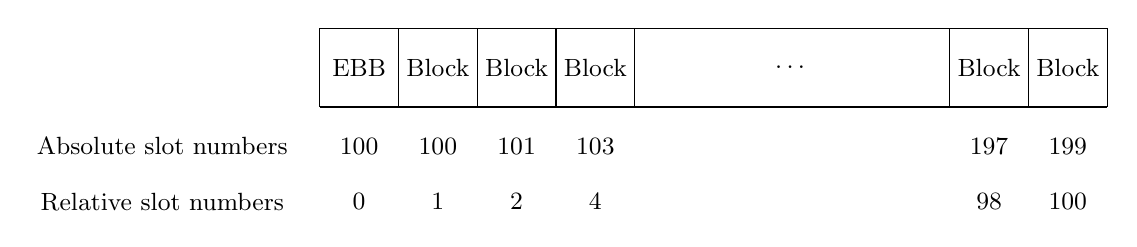
\begin{tikzpicture}
\draw (0, 0) -- (10, 0);
\draw (0, 1) -- (10, 1);

\draw ( 0, 0) -- ( 0, 1);
\draw ( 1, 0) -- ( 1, 1);
\draw ( 2, 0) -- ( 2, 1);
\draw ( 3, 0) -- ( 3, 1);
\draw ( 4, 0) -- ( 4, 1);
\draw ( 8, 0) -- ( 8, 1);
\draw ( 9, 0) -- ( 9, 1);
\draw (10, 0) -- (10, 1);

\draw (0.5, 0.5) node {\small EBB};
\draw (1.5, 0.5) node {\small Block};
\draw (2.5, 0.5) node {\small Block};
\draw (3.5, 0.5) node {\small Block};
\draw (6.0, 0.5) node {\small \ldots};
\draw (8.5, 0.5) node {\small Block};
\draw (9.5, 0.5) node {\small Block};

\draw (-2.0, -0.5) node {\small Absolute slot numbers};
\draw ( 0.5, -0.5) node {\small 100};
\draw ( 1.5, -0.5) node {\small 100};
\draw ( 2.5, -0.5) node {\small 101};
\draw ( 3.5, -0.5) node {\small 103};
\draw ( 8.5, -0.5) node {\small 197};
\draw ( 9.5, -0.5) node {\small 199};

\draw (-2.0, -1.2) node {\small Relative slot numbers};
\draw ( 0.5, -1.2) node {\small 0};
\draw ( 1.5, -1.2) node {\small 1};
\draw ( 2.5, -1.2) node {\small 2};
\draw ( 3.5, -1.2) node {\small 4};
\draw ( 8.5, -1.2) node {\small 98};
\draw ( 9.5, -1.2) node {\small 100};
\end{tikzpicture}
\end{center}
Note that some slots are empty, e.g., 102 and 198 are missing. The first and
lasts slots can be empty too. In practice, it will never be the case that an
entire chunk is empty, but the implementation allows for it.

If we were to pick a chunk size of 1 and store each block in its own file, we
would need millions of files, as there are millions of blocks. When serving
blocks to peer, we would constantly open and close individual block files, which
is very inefficient.

If we pick a very large or even unbounded chunk size, the resulting chunk file
would be several gigabytes in size and keep growing. This would make the
recovery process (\cref{immutable:implementation:recovery}) more complicated and
potentially much slower, as more data might have to be read and
validated.\todo{Other arguments?} Moreover, our current approach of caching
indices per chunk would have to be revised.

In practice, a chunk size of \num{21600} is used, which matches the \emph{epoch
size} of Byron. It is no coincidence that there is (at most) one EBB at the
start of each Byron epoch, fitting nicely in the first relative slot that we
reserve for it. Originally, the Immutable DB called these chunk files
\emph{epoch files}. With the advent of Shelley, which has a different epoch size
than Byron, we decoupled the two and introduced the name ``chunk''.

\paragraph{Dynamic chunk size}

The \emph{chunking} scheme was designed with the possibility of a non-uniform
chunk size in mind. Originally, the goal was to make the chunk size configurable
such that the number of slots per chunk could change after a certain slot.
Similarly, the reserving an extra slot for an EBB would be optional and could
stop after a certain slot, i.e., when the production of EBBs stopped. The
reasoning behind this was to allow the chunk size to change near the transition
from Byron to Shelley. As the slot density goes down by a factor of twenty when
transitioning to Shelley, the number of blocks per chunk file and, consequently,
the chunk size would go down by the same factor, leading to too many, smaller
chunk files. The intention was to configure the chunk size to increase by the
same factor at the start of the Shelley era.

The transition to another era, e.g., Shelley, is dynamic: the slot at which it
happens is determined by on-chain voting and is not certain up to a number of
hours in advance. Making the mapping from slot number to chunk and relative slot
number rely on the actual slot at which the transition happened would complicate
things significantly. It would make the mapping depend on the ledger state,
which determines the current era. This would make an unwanted coupling between
the Immutable DB, storing \emph{blocks}, to the ledger state obtained by
applying these blocks. A reasonable compromise would be to hard-code the change
in chunk size to the estimated transition slot. When the estimate is incorrect,
only a few Byron chunks would contain more blocks than intended or only a few
Shelley chunks would contain fewer blocks than intended.

Unfortunately, due to lack of time, dynamic chunk sizes were not implemented in
time for the transition to Shelley. This means the same chunk size is being used
for the \emph{entire chain}, resulting in fewer blocks per Shelley chunk file
than ideal, and, consequently, more chunk files than ideal.

\paragraph{Indexing by block number}

The problem of too small, too many chunk files described in the paragraph above
is caused by the fact that slot numbers can be sparse and do not have to be
consecutive. \emph{Block numbers} do not have the same problem: they are
consecutive and thus dense, regardless the era of the blockchain. If instead of
indexing the Immutable DB by slot numbers, we indexed it by \emph{block
numbers}, we would not have the problem. Unfortunately, the point type, which is
used throughout the network layer and the consensus layer to identify and look
up blocks, consists of a hash and \emph{slot number}, not a block number.

Either we would have to maintain another index from slot number to block number,
which would require its own chunking scheme based on slot numbers or just one
big file, which has its own downsides. Or, points should be based on block
numbers instead of slot numbers. As points are omnipresent, this change is very
far-reaching. The latter approach carries our preference, but is currently out
of the question. The former is more localised, but the complexity and risks
involved in migrating deployed on-disk databases to the new format do not
outweigh the uncertain benefits.

\subsection{Indices}
\label{immutable:implementation:indices}

As mentioned before, we have on-disk indices for the chunk files for two
purposes:
\begin{enumerate}
\item To map the sparse slot numbers to the blocks that are densely stored in
  the chunk files.
\item To store the information about a block that should be available without
  having to read and deserialise the actual block, e.g., the header offset, the
  header size, the CRC32 checksum, etc.
\end{enumerate}
We use a separate index for each task: the \emph{primary index} for the first
task and the \emph{secondary index} for the second task. Each chunk file has a
corresponding primary index file and secondary index file. Because of a
dependency of the primary index on the secondary index, we first discuss the
latter.

\paragraph{Secondary index}

In the secondary index, we store the information about a block that is needed
before or without having to read and deserialise the block. The secondary index
is an append-only file, like the chunk file, and contains a \emph{secondary
index entry} for each block. For simplicity and robustness, a secondary index
merely contains a series of densely stored secondary index entries with no extra
information between, before, or after them. This avoids needing to initialise or
finalise such a file, which also makes the recovery process simpler
(\cref{immutable:implementation:recovery}). A secondary index entry consists of
the following fields:

\begin{center}
\begin{tabular}{l r}
  field & size [bytes] \\
  \hline
  block offset  & 8 \\
  header offset & 2 \\
  header size   & 2 \\
  checksum      & 4 \\
  header hash   & X \\
  block or EBB  & 8 \\
\end{tabular}
\end{center}

\begin{itemize}
\item The block offset is used to determine at which offset in the corresponding
  chunk file the raw block can be read.

  As blocks are variable-sized, the size of the block also needs to be known in
  order to read it. Instead of spending another 8 bytes to store the block size
  as an additional field, we read the block offset of the \emph{next entry} in
  the secondary index, which corresponds to the block after it. The block size
  can then be computed by subtracting the latter's block offset from the
  former's.

  In case the block is the final block in the chunk file, there is no next
  entry. Instead, the final block's size can be derived from the chunk file's
  size. When reading the final block $B_n$ of the current chunk file, it is
  important to obtain the chunk file size at the right time, before any more
  blocks ($B_{n+1}, B_{n+2}, \ldots$) are appended to the same file, increasing the
  chunk file size. Otherwise, we risk reading the bytes corresponding to not
  just the previously final block $B_n$, but also $B_{n+1}, B_{n+2},
  \ldots$\footnote{In hindsight, storing the block size as a separate field would
  have simplified the implementation.}

  The reasoning behind using 8 bytes for the block offset is the following. The
  maximum block header and block body sizes permitted by the blockchain itself
  are dynamic parameters that can change through on-chain voting. At the time of
  writing, the maximum header size is 1100 bytes and the maximum body size is
  \num{65536} bytes. By multiplying this theoretical maximum block size of
  $\num{1100} + \num{65536} = \num{66636}$ bytes by the chunk size used in
  practice, i.e., \num{21600}, assuming a maximal density of 1.0 in the Byron
  era, we get \num{1439337600} as the maximal file size for a chunk file. An
  offset into a file of that size fits tightly in 4 bytes, but this would not
  support any future maximum block size increases, hence the decision to use 8
  bytes.

\item The header offset and header size are needed to extract the header from a
  block without first having to read and deserialise the entire block, as
  discussed in \cref{serialisation:storage:nested-contents}. These are stored
  per block, as the header size can differ from block to block. The nested
  context is reconstructed by reading bytes from the start of the block, as
  explained in our discussion of the \lstinline!ReconstructNestedCtxt! class in
  \cref{serialisation:storage:nested-contents}.

  Using 2 bytes for the header offset and header size is enough when taking the
  following into account: (so far all types of) blocks start with their header,
  the current maximum header size is \num{1100} bytes, and the header offset is
  relative to the start of the block.

\item As discussed before, to detect silent corruption of blocks, we store a CRC
  checksum of each block, against which the block is verified after reading it.
  This verification can be done without deserialising the block.

  Note that we do not store a checksum of the raw header, which means we do not
  check for silent corruption when streaming headers.\todo{Maybe we should?}

\item The header hash is used for lookups and bounds checking, i.e., to check
  whether the given point's hash matches the hash of the block as the same slot
  in the Immutable DB. By storing it separately, we do not have to read and
  compute the hash of the block's header just to check whether it has the right
  hash.

  The header hash field's size depends on the concrete instantiation of the
  \lstinline!HeaderHash blk! type family. In practice, a 32-byte hash is used.

\item The ``block or EBB'' field is represented in memory as follows:

  \begin{lstlisting}
  data BlockOrEBB =
      Block !SlotNo
    | EBB   !EpochNo
  \end{lstlisting}

  The former constructor represents a regular block with an absolute slot number
  and the latter an EBB (\cref{ebbs}) with an epoch number (since there is only
  a single EBB per epoch). The main reason this field is part of the secondary
  index entry is to implement the \lstinline!iteratorHasNext! method of the
  iterator API (see \cref{immutable:api:iterators}) without having to read the
  next block from disk, as the iterator will keep these secondary index entries
  in memory.

  Both the \lstinline!SlotNo! and \lstinline!EpochNo! types are newtypes around
  a \lstinline!Word64!, hence the 8 on-disk bytes. We omit the tag
  distinguishing between the two constructors in the serialisation because in
  nearly all cases, this information has already been retrieved from the primary
  index, i.e., whether the first filled slot in a chunk is an EBB or
  not.\footnote{In hindsight, having the tag in the serialisation would have
  simplified the implementation.}

\item Because of the fixed size of each field, it was originally decided to
  (de)serialise the corresponding data type using the \lstinline!Binary! class.
  Using CBOR would be more flexible to future changes. This would make the
  encoding variable-sized, which is not necessarily an issue, which will become
  clear in our description of the primary index.

\end{itemize}

\paragraph{Primary index}

The primary index maps the sparse slot numbers to the secondary index entries of
the corresponding blocks in the dense secondary index. As discussed above, the
secondary index entry of a block tells us the offset in the chunk file of the
corresponding block.

The format of the primary index is as follows. The primary index start with a
byte indicating its version number. Next, for each slot, empty or not, we store
the offset at which its secondary index entry starts in the secondary index.
This same offset will correspond to the \emph{end} of the previous secondary
index entry. When a slot is empty, its offset will be the same as the offset of
the slot before it, indicating that the corresponding secondary index entry is
empty.

When appending a new block, we append the previous offset as many times as the
number of slots that was skipped, indicating that they are empty. Next, we
append the offset after the newly appended secondary index entry corresponding
to the new block.

We use a fixed size of 4 bytes to store each offset. As this is an offset in the
secondary index, it should be at least large enough to address the maximal size
of a secondary index file. We can compute this by multiplying the used chunk
size by the size of a secondary index entry: $\num{21600} * (8 + 2 + 2 + 4 + 32
+ 8) = \num{1209600}$, which requires more than 2 bytes to address.

To look up the secondary index entry for a certain slot, we compute the
corresponding chunk number and relative slot number using $\mathsf{chunkNumber}$
and $\mathsf{relativeSlot}$ (we discuss how we deal with EBBs later). Because we
use a fixed size for each offset, based on the relative slot number, we can
compute exactly at which bytes should be read at which offset in the primary
index, i.e., the 4 + 4 bytes corresponding to the offset at the relative slot
and the offset after it. When both offsets are equal, the slot is empty. When
not equal, we now know which bytes to read from the secondary index to obtain
the secondary index entry corresponding to the block in question.

However, as mentioned in \cref{immutable:implementation}, we maintain a cache of
primary indices, which means that they are always read from disk in their
entirety. After a cache hit, looking up a relative slot in the cached primary
index corresponds to a constant-time lookup in a vector.

We illustrate this format with an example primary index below, which matches the
chunk out of the example from \cref{immutable:implementation:chunk-layout}. The
offsets correspond to the blocks on the line below them, where $\emptyset$ indicates an
empty slot. We assume a fixed size of 10 bytes for each secondary index entry.
The offset $X$ corresponds the final size of the secondary index.

\begin{center}
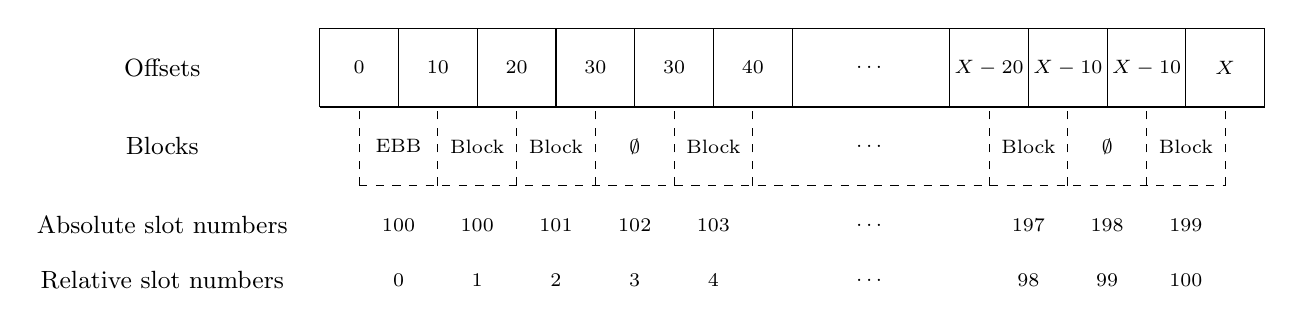
\begin{tikzpicture}
\draw (0, 0)  -- (12, 0);
\draw (0, 1)  -- (12, 1);

\draw ( 0, 0) -- ( 0, 1);
\draw ( 1, 0) -- ( 1, 1);
\draw ( 2, 0) -- ( 2, 1);
\draw ( 3, 0) -- ( 3, 1);
\draw ( 4, 0) -- ( 4, 1);
\draw ( 5, 0) -- ( 5, 1);
\draw ( 6, 0) -- ( 6, 1);
\draw ( 8, 0) -- ( 8, 1);
\draw ( 9, 0) -- ( 9, 1);
\draw (10, 0) -- (10, 1);
\draw (11, 0) -- (11, 1);
\draw (12, 0) -- (12, 1);

\draw (-2.0, 0.5) node {\small Offsets};
\draw ( 0.5, 0.5) node {\scriptsize  0};
\draw ( 1.5, 0.5) node {\scriptsize 10};
\draw ( 2.5, 0.5) node {\scriptsize 20};
\draw ( 3.5, 0.5) node {\scriptsize 30};
\draw ( 4.5, 0.5) node {\scriptsize 30};
\draw ( 5.5, 0.5) node {\scriptsize 40};
\draw ( 7.0, 0.5) node {\scriptsize \ldots};
\draw ( 8.5, 0.5) node {\scriptsize $X - 20$};
\draw ( 9.5, 0.5) node {\scriptsize $X - 10$};
\draw (10.5, 0.5) node {\scriptsize $X - 10$};
\draw (11.5, 0.5) node {\scriptsize $X$};

\draw[dashed] (0.5, -1) -- (11.5, -1);

\draw[dashed] ( 0.5, -1) -- ( 0.5, 0);
\draw[dashed] ( 1.5, -1) -- ( 1.5, 0);
\draw[dashed] ( 2.5, -1) -- ( 2.5, 0);
\draw[dashed] ( 3.5, -1) -- ( 3.5, 0);
\draw[dashed] ( 4.5, -1) -- ( 4.5, 0);
\draw[dashed] ( 5.5, -1) -- ( 5.5, 0);
\draw[dashed] ( 8.5, -1) -- ( 8.5, 0);
\draw[dashed] ( 9.5, -1) -- ( 9.5, 0);
\draw[dashed] (10.5, -1) -- (10.5, 0);
\draw[dashed] (11.5, -1) -- (11.5, 0);

\draw (-2.0, -0.5) node {\small Blocks};
\draw ( 1.0, -0.5) node {\scriptsize EBB};
\draw ( 2.0, -0.5) node {\scriptsize Block};
\draw ( 3.0, -0.5) node {\scriptsize Block};
\draw ( 4.0, -0.5) node {\scriptsize $\emptyset$};
\draw ( 5.0, -0.5) node {\scriptsize Block};
\draw ( 7.0, -0.5) node {\scriptsize \ldots};
\draw ( 9.0, -0.5) node {\scriptsize Block};
\draw (10.0, -0.5) node {\scriptsize $\emptyset$};
\draw (11.0, -0.5) node {\scriptsize Block};

\draw (-2.0, -1.5) node {\small Absolute slot numbers};
\draw ( 1.0, -1.5) node {\scriptsize 100};
\draw ( 2.0, -1.5) node {\scriptsize 100};
\draw ( 3.0, -1.5) node {\scriptsize 101};
\draw ( 4.0, -1.5) node {\scriptsize 102};
\draw ( 5.0, -1.5) node {\scriptsize 103};
\draw ( 7.0, -1.5) node {\scriptsize \ldots};
\draw ( 9.0, -1.5) node {\scriptsize 197};
\draw (10.0, -1.5) node {\scriptsize 198};
\draw (11.0, -1.5) node {\scriptsize 199};

\draw (-2.0, -2.2) node {\small Relative slot numbers};
\draw ( 1.0, -2.2) node {\scriptsize 0};
\draw ( 2.0, -2.2) node {\scriptsize 1};
\draw ( 3.0, -2.2) node {\scriptsize 2};
\draw ( 4.0, -2.2) node {\scriptsize 3};
\draw ( 5.0, -2.2) node {\scriptsize 4};
\draw ( 7.0, -2.2) node {\scriptsize \ldots};
\draw ( 9.0, -2.2) node {\scriptsize 98};
\draw (10.0, -2.2) node {\scriptsize 99};
\draw (11.0, -2.2) node {\scriptsize 100};

\end{tikzpicture}
\end{center}

The version number we mentioned above can be used to migrate indices in the old
format to a newer format, when the need would arise in the future. We do not
include a version number in the secondary index, as both index formats are
tightly coupled, which means that both index files should be migrated together.

One might realise that because the size of a secondary index entry is static,
the primary index could be represented more compactly using a bitmap. This is
indeed the case and the reason for it not being a bitmap is mostly a historical
accident. However, this accident has the upside that migrating to variable-sized
secondary index entries, e.g., serialised using CBOR instead of
\lstinline!Binary! is straightforward.

\paragraph{Lookup}

Having discussed both index formats, we can now finally detail the process of
looking up a block by a point. Given a point with slot $s$ and hash $h$, we need
to go through the following steps to read the corresponding block:

\begin{enumerate}
\item Determine the chunk number $c = \chunkNumber{s}$.
\item Determine the relative slot $\mathit{rs}$ within chunk $c$ corresponding
  to $s$: $\mathit{rs} = \relativeSlot{s}{\mathit{isEBB}}$.

  Note the $\mathit{isEBB}$ argument, which is unknown at this point. Just by
  looking at the slot and the static chunk size, we can tell whether the block
  \emph{could} be an EBB or not: only the very first slot in a chunk (which has
  the same size as a Byron epoch) could correspond to an EBB \emph{or} the
  regular block after it. For all other slots we are certain they cannot
  correspond to an EBB.

  In case the slot $s$ corresponds to the very first slot in the chunk, we will
  have to use the hash $h$ to determine whether the point corresponds to the EBB
  or the regular block in slot $s$.
\item We lookup the offset at $\mathit{rs}$ and the offset after it in the
  primary index of chunk $c$. As discussed, these lookups go through a cache and
  are cheap. We now have the offsets in the secondary index file corresponding
  to the start and end of the secondary index entry we are interested in. If
  both offsets are equal, the slot is empty, and the lookup process terminates.

  In case of a potential EBB, we have to do two such lookups: once for relative
  slot 0 and once for relative slot 1.

\item We read the secondary index entry from the secondary index file. The
  secondary indices are also cached on a per chunk basis. The secondary index
  entry contains the header hash, which we can now compare against $h$. In case
  of a match, we can read the block from the chunk file using the block offset
  contained in the secondary index entry. When the hash does not match, the
  lookup process terminates.

  In case of a potential EBB, the hash comparisons finally tell us whether the
  point corresponds to the EBB or the regular block in slot $s$, or
  \emph{neither} in case both hashes do not match $h$.
\end{enumerate}

\subsection{Recovery}
\label{immutable:implementation:recovery}

Because of the specific requirements of the Immutable DB and the expected write
patterns, we can use a much simpler recovery scheme than traditional database
systems. Only the immutable, append-only part of the chain is stored, which
means that data inconsistencies (e.g., because of a hard shutdown) are most
likely to happen at the end of the chain, i.e., in the last chunk and its
indices. We can simply truncate the chain in such cases. As we maintain some
overlap with the Volatile DB\todo{link}, blocks truncated from the end of the
chain are likely to still be in the Volatile DB, making the recovery process
unnoticeable. If the overlap is not enough and the truncated blocks are not in
the Volatile DB, they can simply be downloaded again.

There are two modes of recovery:
\begin{enumerate}
\item Validate the last chunk: this is the default mode when opening the
  Immutable DB. The last chunk file and its indices are validated. This will
  detect and truncate append operations that did not go through entirely, e.g.,
  a block that was only partially appended to a chunk file, or a block that was
  appended to one or both of the indices, but not to the chunk file.

  When after truncating a chunk file, the chunk file becomes empty, we validate
  the chunk file before it. In the unlikely case that that chunk file has to be
  truncated and ends up empty too, we validate the chunk file before it and so
  on, until we reach a valid block or the database is empty.

\item Validate all chunks: this is the full recovery mode that is triggered by a
  dirty shut down, caused by a missing or corrupted file (e.g., a checksum
  mismatch while reading), or because the node itself was not shut down
  properly.\todo{In the latter case, validating the last would be enough} We
  validate all chunk files and their indices, from oldest to newest. When a
  corrupt or missing block is encountered, we truncate the chain to the last
  valid block before it. Trying to recover from a chain with holes in it would
  be terribly complex, we therefore do not even try it.

\end{enumerate}
In both recovery modes, chunks are validated the same way, which we will shortly
describe. When in full recovery mode, we also check whether the last block in a
chunk is the predecessor of the first block in the next chunk, by comparing the
hashes. This helps sniff out a truncated chunk file that is not the final one,
causing a gap in the chain.

Validating a chunk proceeds as follows:
\begin{itemize}
\item In the common case, the chunk file and the corresponding primary and
  secondary index files will be present and all valid. We optimise for this
  case.\footnote{Unlike in other areas, where we try to maintain that the
  average case is equal to the worst case.}

\item The secondary index contains a CRC32 checksum of each block in the
  corresponding chunk (see \cref{immutable:implementation:indices}), we extract
  these checksums and pass them to the \emph{chunk file parser}.

\item The chunk file parser will try to deserialise all blocks in a chunk file.
  When a block fails to deserialise, it is treated as corrupt and we truncate
  the chain to the last valid block before it. Each raw block is also checked
  against the CRC32 checksum from the secondary index, to detect corruptions
  that are not caught by deserialising, e.g., flipping a bit in a
  \lstinline!Word64!, which can remain a valid, yet corrupt
  \lstinline!Word64!.\footnote{One might think that deserialising the blocks is
  not necessary if the checksums all match. However, the chunk file parser also
  the corresponding secondary index, which is used to validate the on-disk one.
  For this process deserialisation is required.}

  When the CRC32 checksum is not available, because of a missing or partial
  secondary index file, we fall back to the more expensive validation of the
  block based on its cryptographic hashes to detect silent corruption. This type
  of validation is block-dependent and provided in the form of the
  \lstinline!nodeCheckIntegrity! method of the \lstinline!NodeInitStorage!
  class. This validation is implemented by hashing the body of the block and
  comparing it against the body hash stored in the header, and by verifying the
  signature of the header.

  When the CRC32 checksum \emph{is} available, but does not match the one
  computed from the raw block, we also fall back to this validation, as we do
  not know whether the checksum or the block was corrupted (although the latter
  is far more likely).

  The chunk file parser also verifies that the hashes line up within a chunk, to
  detect missing blocks. It does this by comparing the ``previous hash'' of each
  block with the previous block's hash.

  The chunk file parser returns a list of secondary index entries, forming
  together the corresponding secondary index.

\item The chunk file containing the blocks is our source of truth. To check the
  validity of the secondary index, we check whether it matches the secondary
  index returned by the chunk file parser. If there is a mismatch, we overwrite
  the entire secondary index file using the secondary index returned by the
  chunk file parser.

\item We can reconstruct the primary index from the secondary index returned by
  the chunk file parser. When the on-disk primary index is missing or it is not
  equal to the reconstructed one, we (over)write it using the reconstructed one.

\item When truncating the chain, we always make sure that the resulting chain
  ends with a block, i.e., a filled slot, not an empty slot. Even if this means
  going back to the previous chunk.

\end{itemize}

We test the recovery process in our \lstinline!quickcheck-state-machine! tests
of the Immutable DB. In various states of the Immutable DB, we generate one or
more random corruptions for any of the on-disk files: either a simple deletion
of the file, a truncation, or a random bitflip. We verify that after restarting
the Immutable DB, it has recovered to the last valid block before the
truncation.

Additionally, in those same tests, we simulate file-system errors during
operations. For example, while appending a block, we let the second disk write
fail. This is another way of testing whether we can correctly recover from a
write that was aborted half-way through.
